% v2-acmtog-sample.tex, dated March 7 2012
% This is a sample file for ACM Transactions on Graphics
%
% Compilation using 'acmtog.cls' - version 1.2 (March 2012), Aptara Inc.
% (c) 2010 Association for Computing Machinery (ACM)
%
% Questions/Suggestions/Feedback should be addressed to => "acmtexsupport@aptaracorp.com".
% Users can also go through the FAQs available on the journal's submission webpage.
%
% Steps to compile: latex, bibtex, latex latex
%
% For tracking purposes => this is v1.2 - March 2012
\documentclass{acmtog} % V1.2

%\acmVolume{VV}
%\acmNumber{N}
%\acmYear{YYYY}
%\acmMonth{Month}
%\acmArticleNum{XXX}
%\acmdoi{10.1145/XXXXXXX.YYYYYYY}

\let\oldquote\quote
\let\endoldquote\endquote
\renewenvironment{quote}[2][]
  {\if\relax\detokenize{#1}\relax
     \def\quoteauthor{#2}%
   \else
     \def\quoteauthor{#2~---~#1}%
   \fi
   \oldquote}
  {\par\nobreak\smallskip\hfill(\quoteauthor)%
   \endoldquote\addvspace{\bigskipamount}}

\acmVolume{1}
\acmNumber{1}
\acmYear{2018}
\acmMonth{March}
\acmArticleNum{1}
%\acmdoi{10.1145/1559755.1559763}
\makeatletter
\def\runningfoot{\def\@runningfoot{}}
\def\firstfoot{\def\@firstfoot{}}
\makeatother



\begin{document}

\markboth{Experimental Sentiment Analysis on Twitter}{A Real Time Stream and Big Data Process}

\title{Sentiment Analysis on Twitter : Effect of a Social Network} % title

\author{Mohamed Ben Hamdoune {\upshape and} Yannis Tannier
\affil{University of Paris-Descartes}
% NOTE! Affiliations placed here should be for the institution where the
%       BULK of the research was done. If the author has gone to a new
%       institution, before publication, the (above) affiliation should NOT be changed.
%       The authors 'current' address may be given in the "Author's addresses:" block (below).
%       So for example, Mr. Fogarty, the bulk of the research was done at UIUC, and he is
%       currently affiliated with NASA.
}

\category{I.3.7}{Database}{Big Data and Real Stream}[Cloud Computing]
\category{I.3.5}{Social Media Analytics}{Apache Spark and Hadoop}[Machine Learning]

\terms{Twitter, Psychological Profil}

\keywords{Natural Languages Processing, Contradiction Analysis, Opinon Mining, Classification, Text Mining}

\acmformat{Mohamed Ben Hamdoune, Yannis Tannier. 2018. Sentiment Analysis for Twitter : Effect of a Social Network.}

\maketitle

\begin{bottomstuff}
Jason Scott Sadofsky acknowledges a  Jason Scott, is an American archivist, historian of technology, and filmmaker. Archive Team is a group dedicated to preserving digital history that was founded by Jason Scott in 2009.
https://www.archiveteam.org/
Data collected for where on the website of The Archive Team
\end{bottomstuff}


\begin{abstract}
Our purpose is to build a powerful platform \cite{Baltas17} for real-time data analysis of tweets on twitter trends. We also want to analyse all the tweets of 2017 based on a downloaded sample of data (average of 6To).
All this data analysis will be accessible via a web interface that will be developed.
We want to build a powerful system of sentiments analysis by making a database structure of tweets which is relevant to impacts and effects. The system should provide a faster way to execute Machine Learning methodologies behind data extracted from Twitter.
Analysis news actuality by getting an analysis on actual trends with real stream data.
Build an efficient web interface to get results easily.
Build a system without false accounts and keep a control on data continuously.
\end{abstract}

\section{Introduction}
The main subject is Sentiment Analysis on Twitter, a microblogging platform where people can easily share their thought on anything and their habits too. We have a lot of publications on sentiment analysis but not so much research about impacts and their effect on society.
The maximum characters are 140 which can be a good thing for the process of analysis because it will make it faster in a way to perform on small messages but in the other hand we should pay attention on precision of results.
Event it’s an enormously continuous stream of data, Twitter is a good extra sentiment though an online community.  
Finally, how to optimize all those streaming data and build a web interface for users who want to get data.
Our project will use many methodologies from Machine Learning like unsupervised methods to make a classification of sentiments, and supervised method to predicate psychological profile.
Finally, one big step will be and efficient system about control of massive data incoming, a check on false account and spam messages that will destroy our results for example.
 
\begin{quote}{Jeffrey Zeldman}
“The best way to engage honestly with the marketplace via Twitter is to never use the words "engage," "honesty," or "marketplace." 
\end{quote}

First, we will talk \cite{Meisheri17} about scripts using Pyspark with Scikit-learn and TextBlop. 
Scikit-learn allows us a a lots simple and efficient tools for data mining and data analysis, it’s accessible to everybody and reusable in various contexts. It’s Open source and commercially usable.
TextBlob is a library fro processing textual data. It provides a simple API for diving into common natural language processing (NLP) tasks such as sentiment analysis, classification, translation, and more. TextBlop use Google translate for sentences that are not in English, so in free and anonymous usage are limited 1000 words/day which is why we could not have analysed every tweet on the database.
The Spark Python API (PySpark) exposes the Spark programming model to Python. We used it because it simpler and we have a gain of productivity against language such as Scala or Java. Python is dynamically type, so RDDs can hold objects of multiple types.
To run all those libraries, we used Amazon EMR, an Amazon EMR release is a set of open-source applications from the big-data ecosystem. Each release comprises different big-data applications, components, and features that we selected to have Amazon EMR installed and configured when we create a cluster (more here). 
For the real-stream part, we created a module for Data Stream with Kinesis MQTT (exemple). We used a StreamListener that will permanently get data from Twitter and with TextBlop we run an analysis on each tweet and sum all of them.

MQTT is a publish-subscribe messaging protocol based on the TCP / IP protocol, it was originally developed by Andy Stanford-Clark (IBM) and Arlan Nipper (EurtoTech), then offered to the Open Source community (For information, MQTT v3.1.1 is now an OASIS standard).
POMS (Profile Of Mood States) is a psychological rating scale used for calculating the mood state score, the result depends on the values of 65 adjectives. For our project we reorganized the adjectives in two ways, first in 3 categories: Positive, Negative and Neutral, second way in 5 categories: Joy, Surprised, Fear, Angry, Sadness. More about the way to calculate POMS adjectives, click here.
We developped the website using React.js, we could design simple views for each state in our application, and React efficiently update and render just the right components when your data changes.
Text from tweets are inherently noisy. They contain twitter specific words along with hashtags and username mentions. Cleaning the text before further processing helps to generate better features and semantics.

\begin{figure*}[t]
\centerline{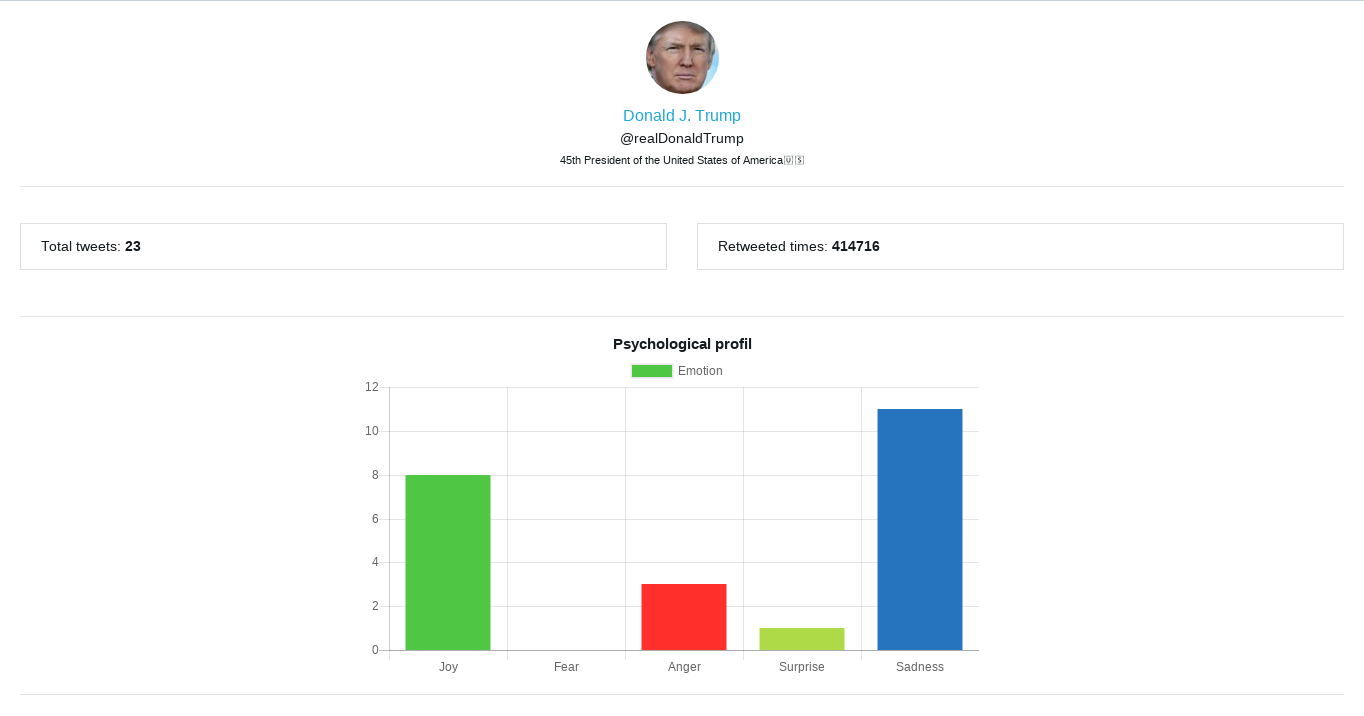
\includegraphics[height=0.5\textwidth]{trump.png}}
\caption{Results predicted by our models with Donald John Trump (born June 14, 1946), the 45th and current President of the United States.}
  \label{fig:trump_results}
\end{figure*}

The data for this task consists of tweets across various domains, classified into four emotions : joy, sadness, anger and fear. The training data additionally carries a real-valued score between 0 and 1 per tweet, indicating the degree of the emotion (that the tweet is classified as) the present in the tweet.
A very quick presentation of all steps in the project:
\begin{enumerate}
\item Fetch data with API (main language we will use is Python), manage collections of stream data.
\item Pre-processing on data with Spark.
\item Build multiple module.
\item Analysis those data with multiple methods of machine learning.
\item Web interface.
\end{enumerate}


\section{Application area:Predicting Psychological Profil}
\label{sec:application area}
%
\looseness-1A few researchers have addressed the issue of realistic
human iris synthesis. Lefohn et al. blend several textures created by an
artist, each containing some eye feature. Other image-based approaches
have been proposed by Cui et al., Wecker et~al., and Makthal and Ross.
Essentially, they decompose a set of iris images using techniques such
as principal component analysis, multiresolution and wavelets, and
Markov random fields, and recombine the obtained data to generate new
images of irises. Zuo and Schmid created a fiber-based 3D model of the
iris. Lam and Baranoski introduced a predictive light transport model
for the human iris, which computes the spectral responses of iridal
tissues described by biophysical parameters. Fran\c{c}ois et~al.
estimate iris height maps from gray-scale images. All these approaches
use stationary pupil sizes.

\section{Previous work}
\label{sec:previous review}

We now turn our attention to the following interesting question: whether the sub-jective data that exist on the web carry useful information. Information can be thought of as data that reduce our uncertainty about some subject. According to this view, the diversity and pluralism of information on different topics can have a rather negative role. It is well understood, that true knowledge is being described by facts, rather than subjective opinions. However, this diversity in opinions, when analyzed, may deliver new information and contribute to the overall knowledge of a subject matter. This is especially true when the object of our study is the attitude of people. In this case, opinion ative data can be useful in order to uncover the distribution of sentiments across time, or different groups of people.

\section{Empirical study}
\label{sub:empirical}

The World Wide Web (Web, for short), is a distributed information system based on hypertext. Web interfaces to databases have become very important. After outlining several reasons for interfacing databases with the Web, we provide an overview of Web Technology. We then outline techniques for building Web interfaces to databases.

\subsection{Implementation}
\label{subsub:implementation}
%
The term data mining refers loosely to process of semiautomaticcally analyzing large databases to find useful patterns. Like knowledge discovery in artificial intelligence (also called machine learning) or statistical alaysis, we use data mining to discover rules and patterns from data. However, data mining differs from machine learning and statistics in that it deals with large volumes of data, stored primarily on disk. That is, data mining deals with “knowledge discovery in databases”. Some types of knowledge discovered from a database can be represented by a set of rules. The following is an example of a rule, stated informally: “Donald Trump with his totals of retweets incomes are greater than the average with the most sadly effects on users”. Of course such riles are not universally true, and have degrees of “support” and “confidence”, as we shall see. Other types of knowledge are represented by equations relating different variables to each other, or by other mechanisms for predicting outcomes when the values of some variables are known. 
There are a variety of possible types of patterns that may be useful, and different techniques are used to find different types of patterns. Usually there is a manual component to data mining, consisting of preprocessing data to a form acceptable to the algorithms and postprocessing of discovered patterns. For this reasin, data mining is really a semiautomatic process in real life. 
The mode widely used applications are those that requires some sort of prediction. In our case, we want to predict emotions and sentiments, then a psychological profil. 
Prediction is one of the mort important types of data mining. We outline what is classification, study techniques for building one type of classifiers, called decision-tree classifiers, and then study other predicition techniques.
Abstractly, the classification problem is this: Given that user belong to the archive, and given his tweet. We use a given instances (called training instances) of items along with the classes to which they belong, the problem is to predict the class (in our study it is a sentiment or an emotion) to which a new item belongs.

\section{Analysis}
\label{sec:analysis}
We have used the following technologies for a number of reasons. Hadoop assumes that conventional approaches (consisting of developing ever more powerful centralized systems) have technical and financial limitations.
The development of distributed systems consisting of machines or nodes, relatively affordable (commodity hardware) and scaling out is an alternative from a technical and financial point of view
A distributed system comprising tens, hundreds or thousands of nodes will regularly be confronted with hardware and / or software failures.
Google has developed the Google File System (GFS), ancestor of the Hadoop Disreated File System (HDFS) and The MapReduce Approach.
MapReduce is a programming model designed specifically to read, milk and write very large volumes of data. A Hadoop program usually implements both map tasks and reduce tasks.

Hadoop is particularly effective for dealing with problems that have one or more of the following characteristics:
Volume of data to store or process very important.
Need to perform processing on all data (batch rather than transactional, therefore).
Heterogeneous data in terms of origin, structure, and format (JSON)
Execute the tasks of a Hadoop job in parallel, without a pre-established order.
A Hadoop cluster is made up of tens, hundreds, or thousands of nodes. It is the addition of the storage and processing capacities of each of these nodes which makes it possible to offer a storage space and a computing power yet to handle data volumes of several To or Po.
To improve the performance of a read / write cluster, Hadoop's file management system, HDFS, writes and reads files in blocks of 64 MB or 128 MB. Working on such large blocks maximizes data transfer rates by limiting search time on hard drives (seek time).
// Input file graph and block
MapReduce is a programming model designed specifically to read, process and write very large volumes of data. A Hadoop program usually implements both map tasks and reduce tasks.
A Hadoop program is usually divided into three parts:
The driver, which runs on a client machine, is responsible for configuring the job and submitting it for execution.
The map is responsible for reading and processing data stored on disk.
The reducer is responsible for consolidating the results from the map and write them on disk.

\subsection{Data Preprocessing}
\label{subsec:data_pre}
Ok

\section{Discussion}
\label{sec:results}

Hence, the difference between Apache Storm vs Spark Streaming shows that Apache Storm is a solution for real-time stream processing. But Storm is very complex for developers to develop applications. There are very limited resources available in the market for it.
Storm can solve only one type of problem i.e Stream processing. But the industry needs a generalized solution which can solve all the types of problems. For example Batch processing, stream processing interactive processing as well as iterative processing. Here Apache Spark comes into limelight which is a general purpose computation engine. It can handle any type of problem. Apart from this Apache Spark is much too easy for developers and can integrate very well with Hadoop.

Apache Spark is an in-memory distributed data analysis platform-- primarily targeted at speeding up batch analysis jobs, iterative machine learning jobs, interactive query and graph processing.
One of Spark's primary distinctions is its use of RDDs or Resilient Distributed Datasets. RDDs are great for pipelining parallel operators for computation and are, by definition, immutable, which allows Spark a unique form of fault tolerance based on lineage information. If you are interested in, for example, executing a Hadoop MapReduce job much faster, Spark is a great option (although memory requirements must be considered).
Apache Storm is focused on stream processing or what some call complex event processing. Storm implements a fault tolerant method for performing a computation or pipelining multiple computations on an event as it flows into a system. One might use Storm to transform unstructured data as it flows into a system into a desired format.
Storm and Spark are focused on fairly different use cases. The more "apples-to-apples" comparison would be between Storm Trident and Spark Streaming. Since Spark's RDDs are inherently immutable, Spark Streaming implements a method for "batching" incoming updates in user-defined time intervals that get transformed into their own RDDs. Spark's parallel operators can then perform computations on these RDDs. This is different from Storm which deals with each event individually.
One key difference between these two technologies is that Spark performs Data-Parallel computationswhile Storm performs Task-Parallel computations. Either design makes tradeoffs that are worth knowing. I would suggest checking out these links.

\section{Conclusion}
\label{sec:conclusion}
%
We have presented new models for realistic renderings of the human iris
and pupil. Our physiologically-based model of the pupil light reflex
combines and extends theoretical results from the Mathematical Biology
field with experimental data collected by several researchers. The
resulting model is expressed in terms of a nonlinear delay-differential
equation that describes the changes in the pupil diameter as function of
the environment lighting. Our model is also original in the sense that
it can simulate individual differences with respect to light
sensitivity. As all parameters of our models were derived from
experimental data, they correctly simulate the actual behavior of the
human iris and pupil. They also produce high-fidelity appearance
effects, which can be used to create\break real-time predictive
animations of the pupil and iris under variable lighting conditions. We
have validated our models through comparisons of our simulated results
against videos and photographs captured from human irises. The quality
of these simulations qualitatively matched the actual behaviors of human
pupils and irises.

To the best of our knowledge, ours is the first physiologically-based
model for simulating pupil light reflex presented in the graphics
literature. It is also the first practical model (providing actual
coefficient values) in the literature for simulating the dynamics of
pupil and iris under variable lighting conditions, and the first
integrated model in all of the literature to consider individual
variability in pupil diameter using general equations for latency and
velocity. Our image-based model for iridal pattern deformation is also
the first model of its kind in the graphics literature.\vskip21pt

% Start of "Sample References" section
\section{References}

\begin{acks}
We are grateful to the following people for resources,discussions and suggestions: Jason Scott(Archivist),Diana Yuan (Co-Founder & Vice President, Talent & Operations from Indico).
\end{acks}


% Bibliography
\bibliographystyle{ACM-Reference-Format-Journals}
\bibliography{publication-bibfile}

                                % Sample .bib file with references that match those in
                                % the 'Specifications Document (V1.5)' as well containing
                                % 'legacy' bibs and bibs with 'alternate codings'.
                                % Gerry Murray - March 2012

\end{document}
% End of v2-acmtog-sample.tex (March 2012) - Gerry Murray, ACM
